% ******************************* Thesis Appendix A ****************************
\setcounter{chapter}{9}
\chapter*{Anexo} 
\addcontentsline{toc}{chapter}{Anexo}
\setcounter{figure}{0}
\setcounter{table}{0}
\setcounter{section}{0}

\graphicspath{{Appendix/Figs/}}

\lstinputlisting[caption={circos.conf},label={circos.conf}]{scripts/circos.conf}

\lstinputlisting[caption={histogram.conf},label={histogram.conf}]{scripts/histogram.conf}

\lstinputlisting[caption={links.conf},label={inks.conf}]{scripts/links.conf}

\setlength{\oddsidemargin}{-1cm}


\begin{landscape}
    \begin{figure}[htbp!] 
        \centering    
        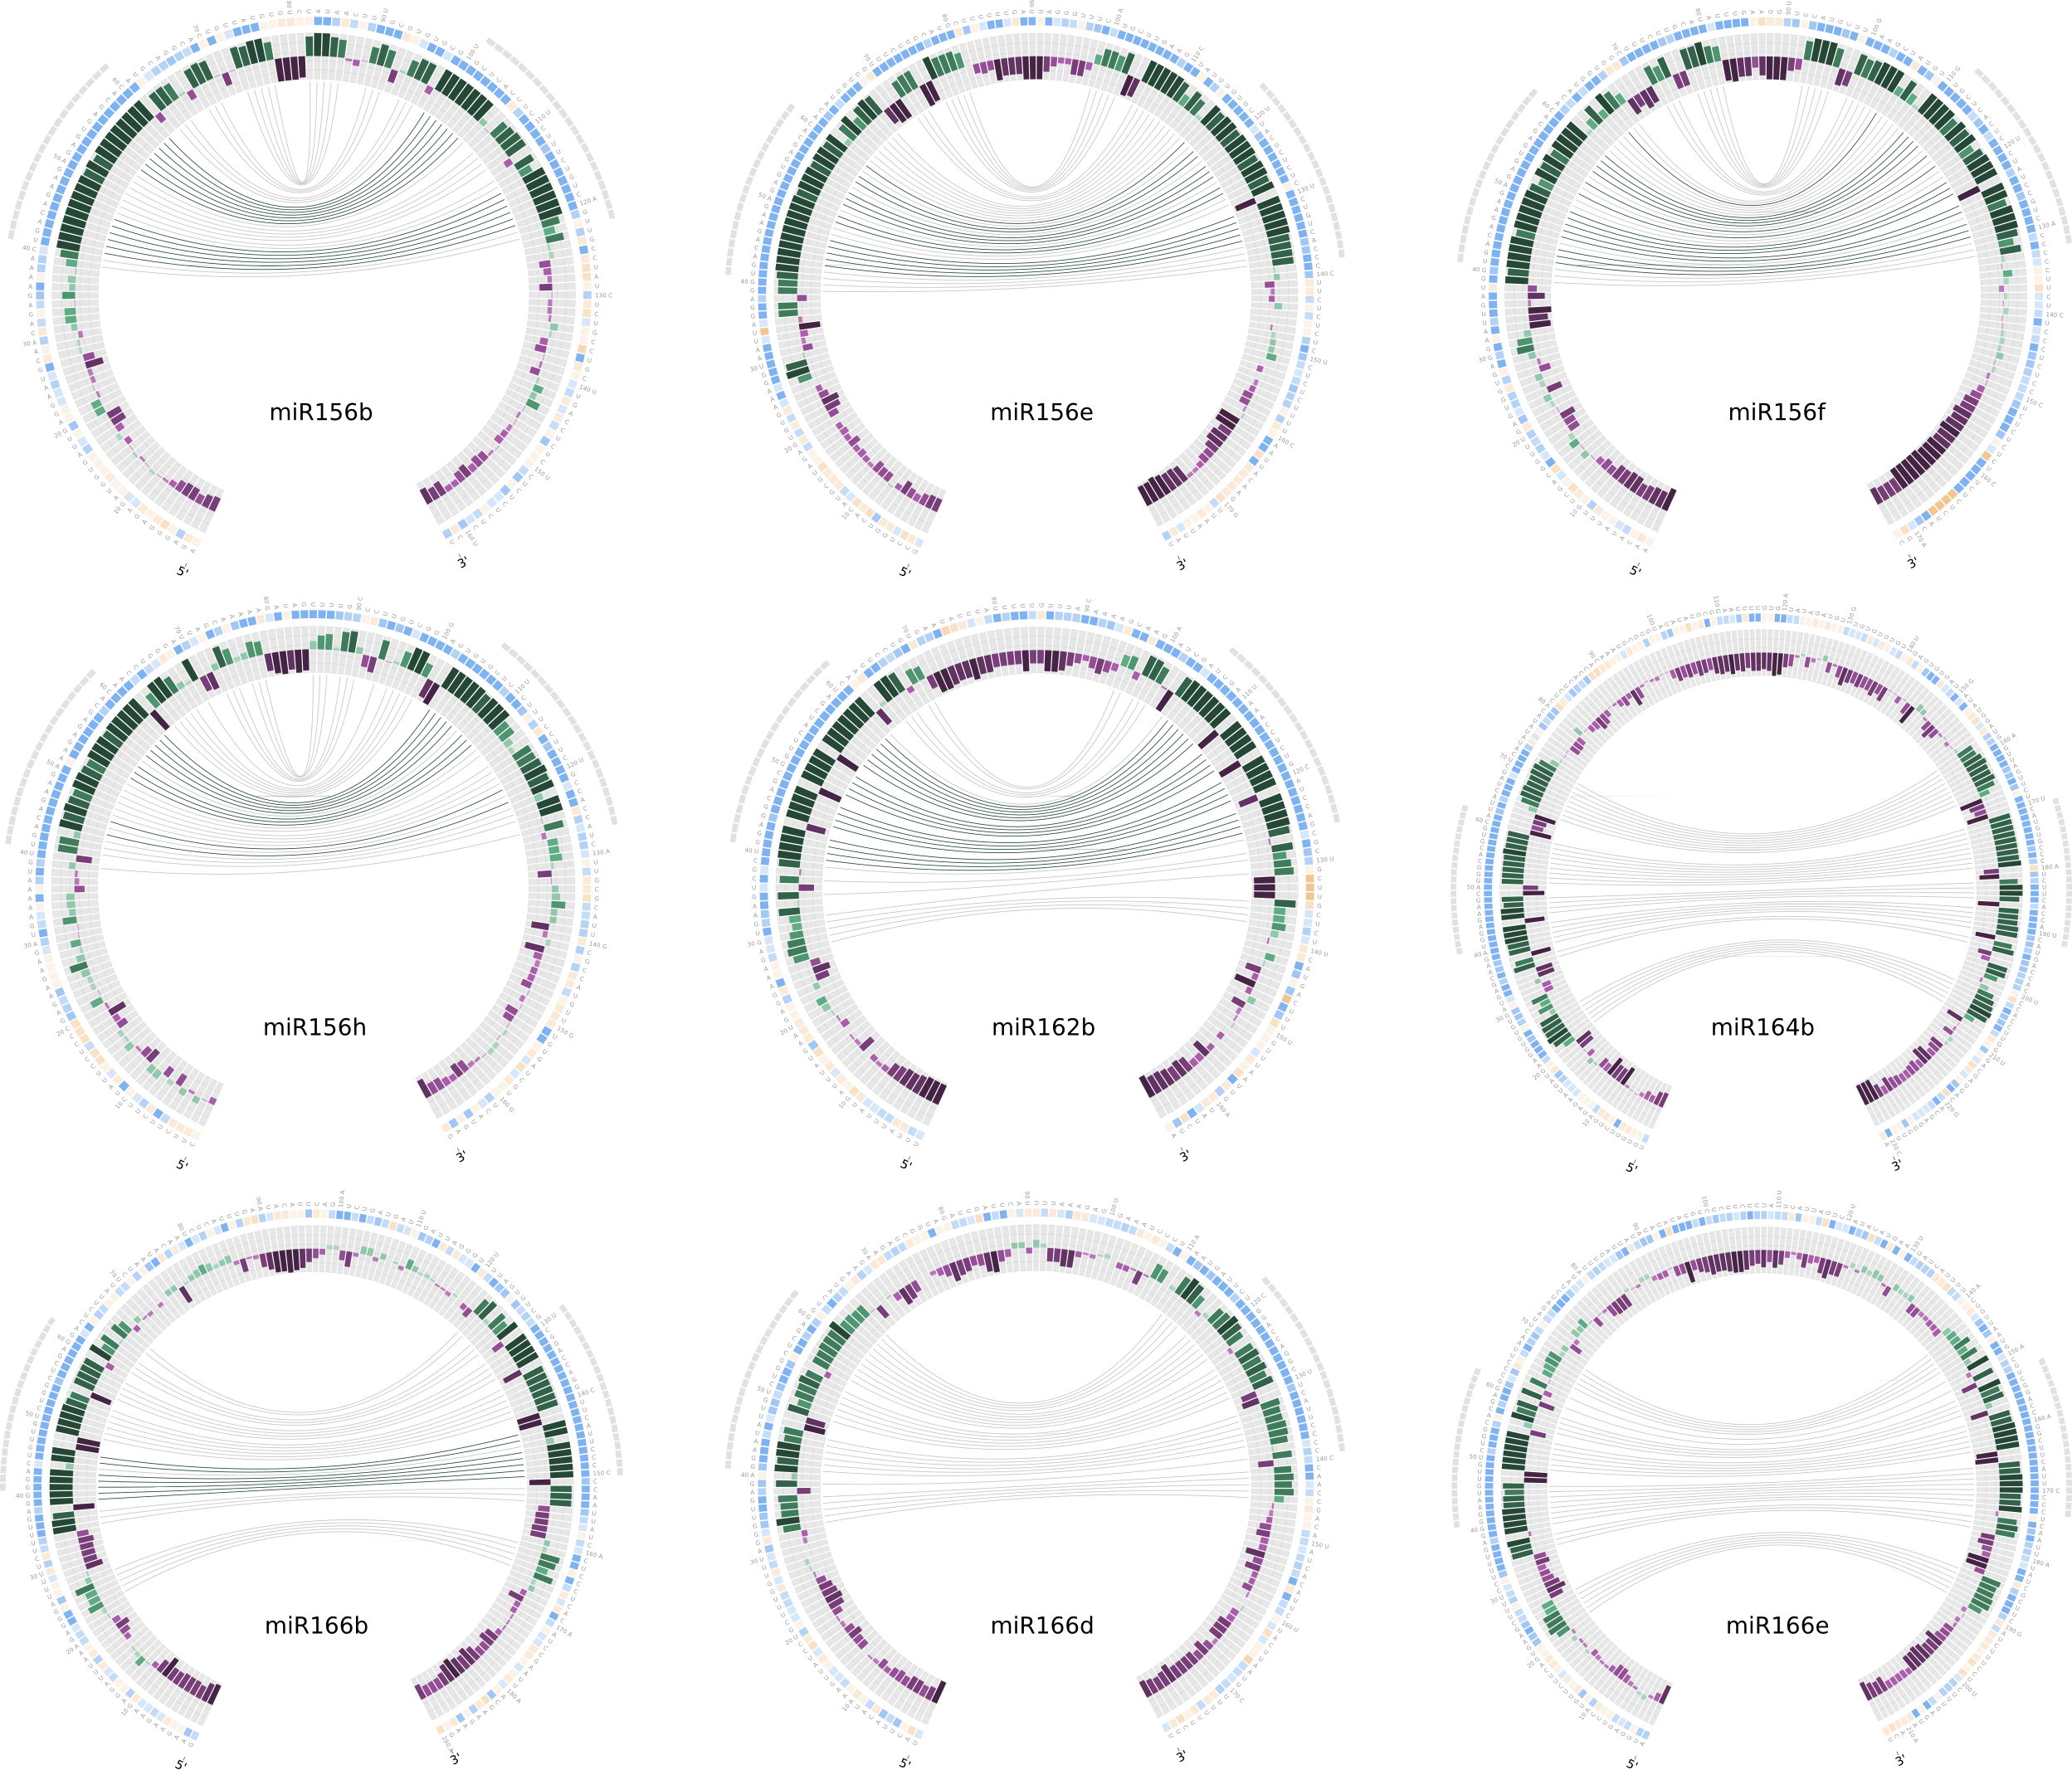
\includegraphics[width=1.4\textwidth]{circos_all_01.png}
        \caption[Circos de dicotiledóneas (en más de 20 especies). 1/5]{
        \textbf{Circos de dicotiledóneas donde se detectan ortólogos en más de 20 especies de las 30 analizadas.}
        Fig 1/5.
        }
        \label{fig:circos_all_01}
    \end{figure}
\end{landscape}

\begin{landscape}
    \begin{figure}[htbp!] 
        \centering    
        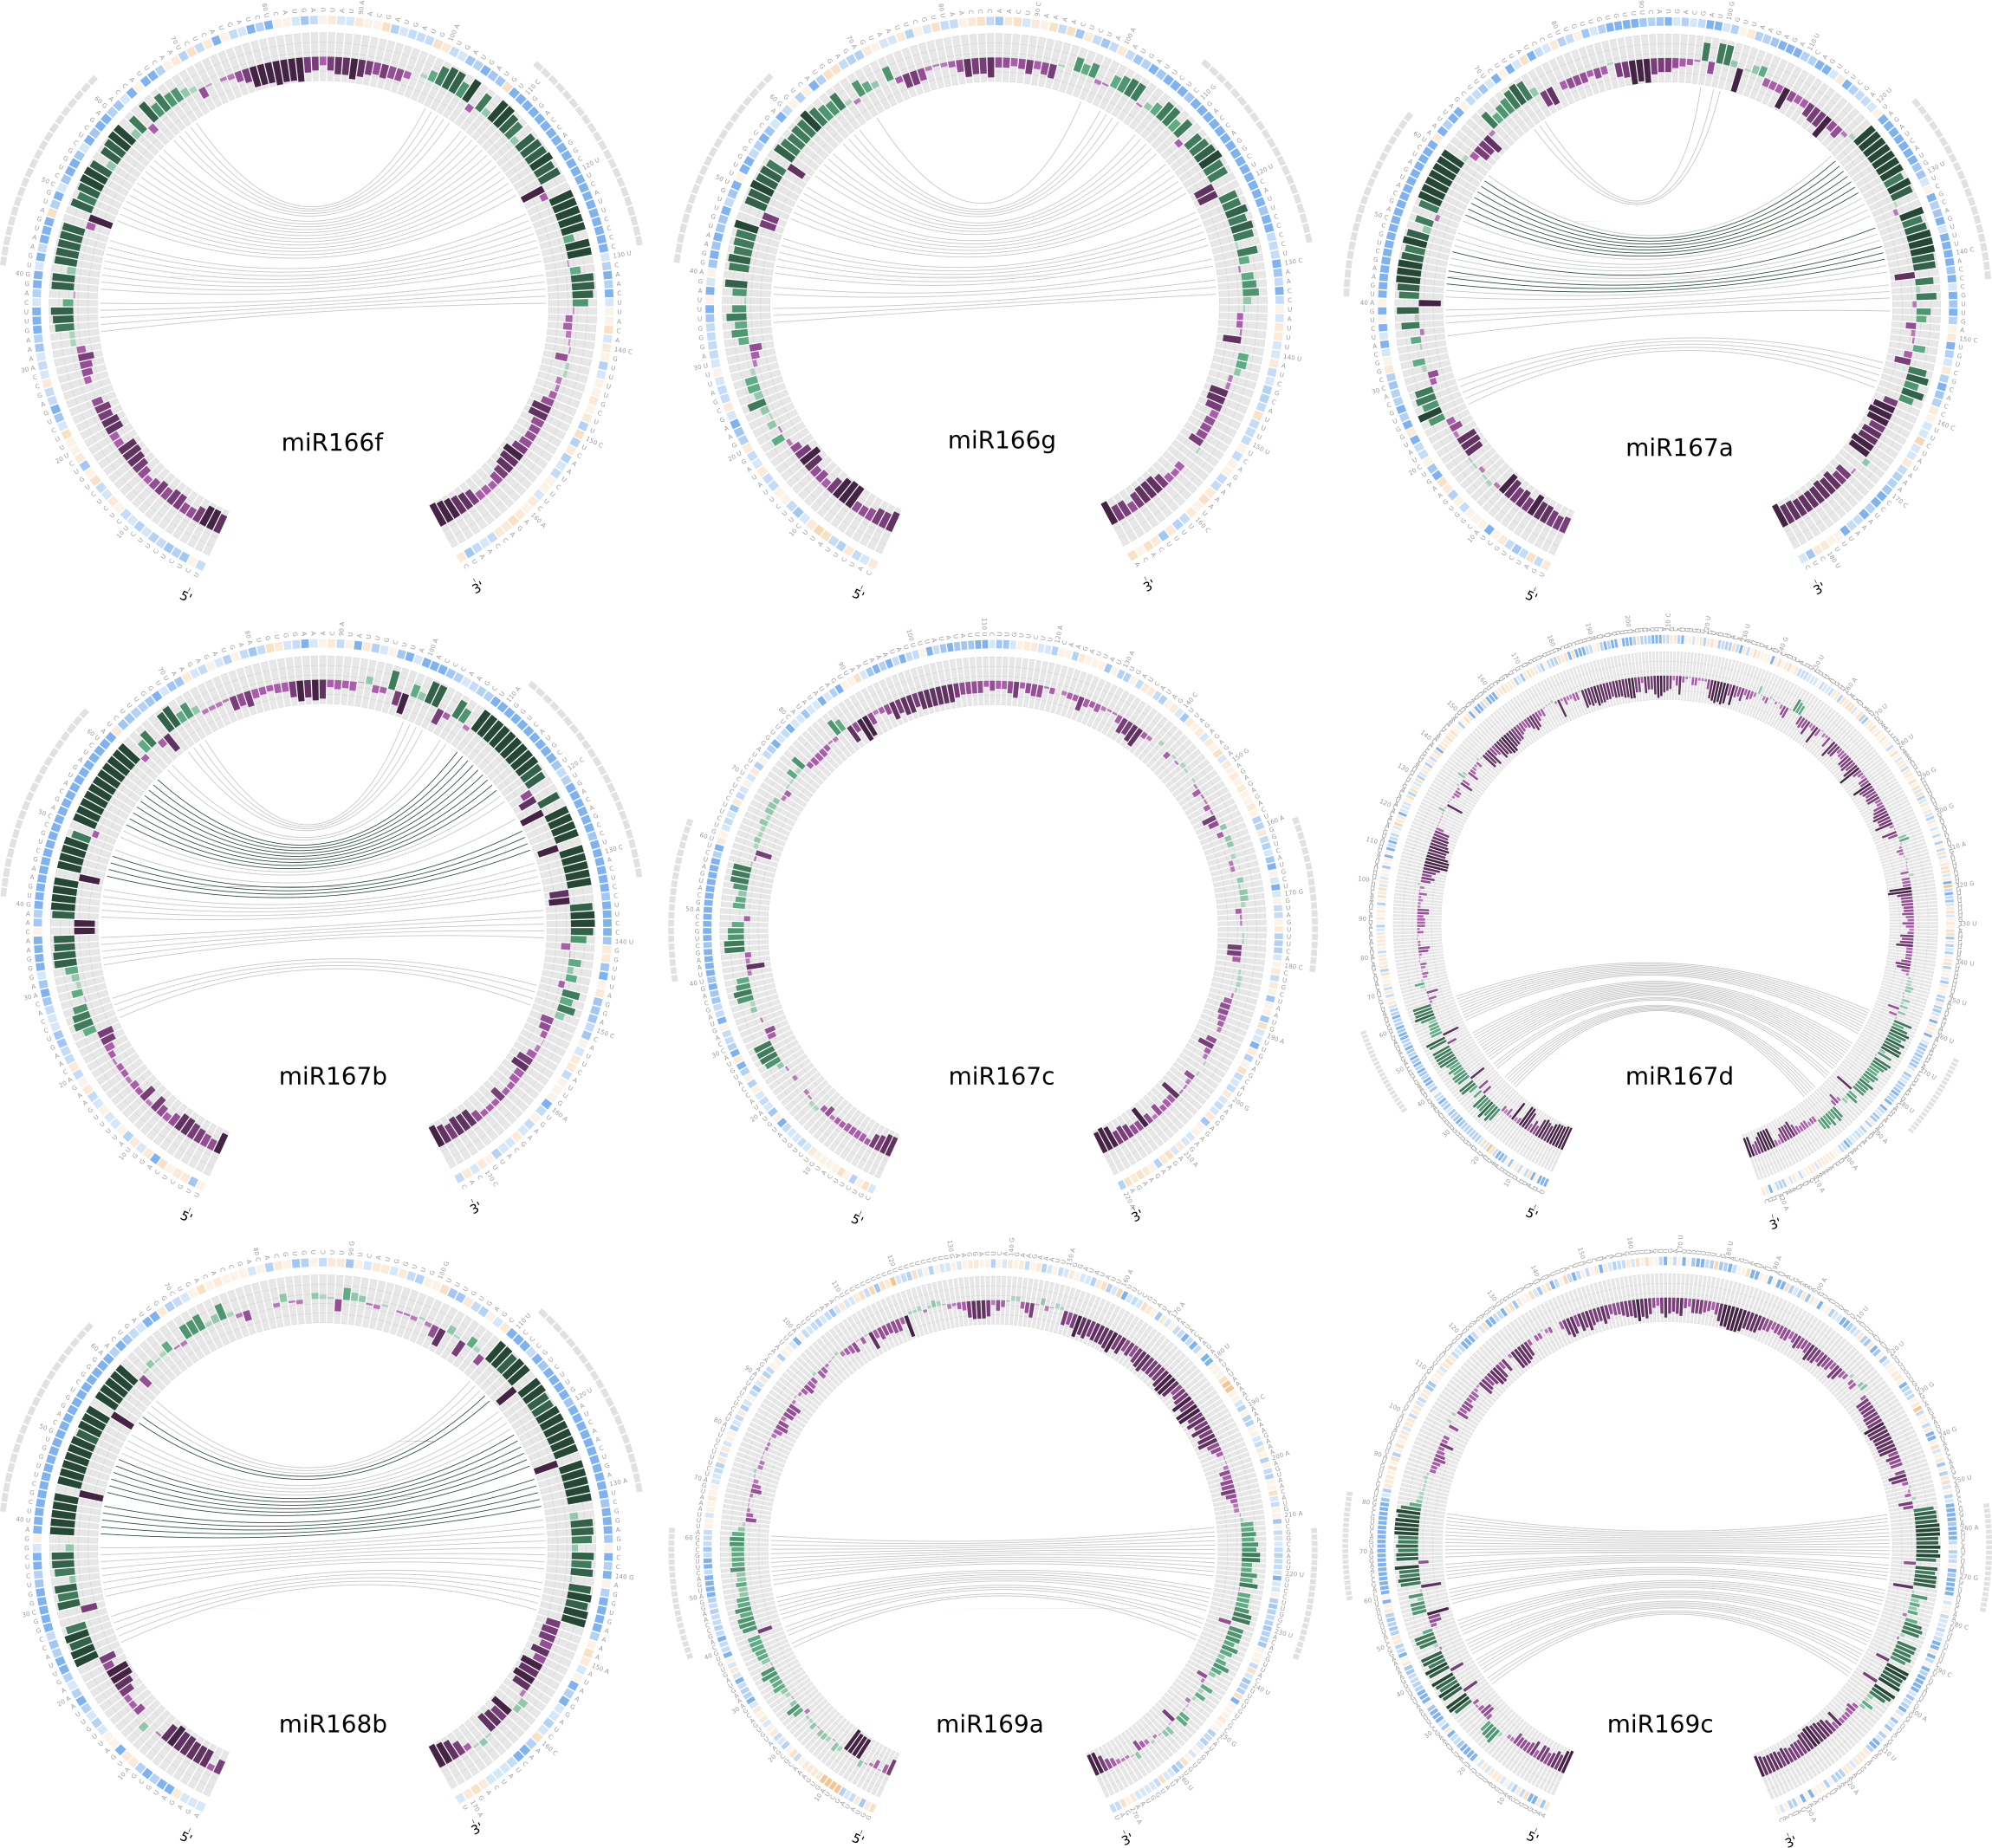
\includegraphics[width=1.3\textwidth]{circos_all_02.png}
        \caption[Circos de dicotiledóneas (en más de 20 especies). 2/5]{
        \textbf{Circos de dicotiledóneas donde se detectan ortólogos en más de 20 especies de las 30 analizadas.}
        Fig 2/5.
        }
        \label{fig:circos_all_02}
    \end{figure}
\end{landscape}

\begin{landscape}
    \begin{figure}[htbp!] 
        \centering    
        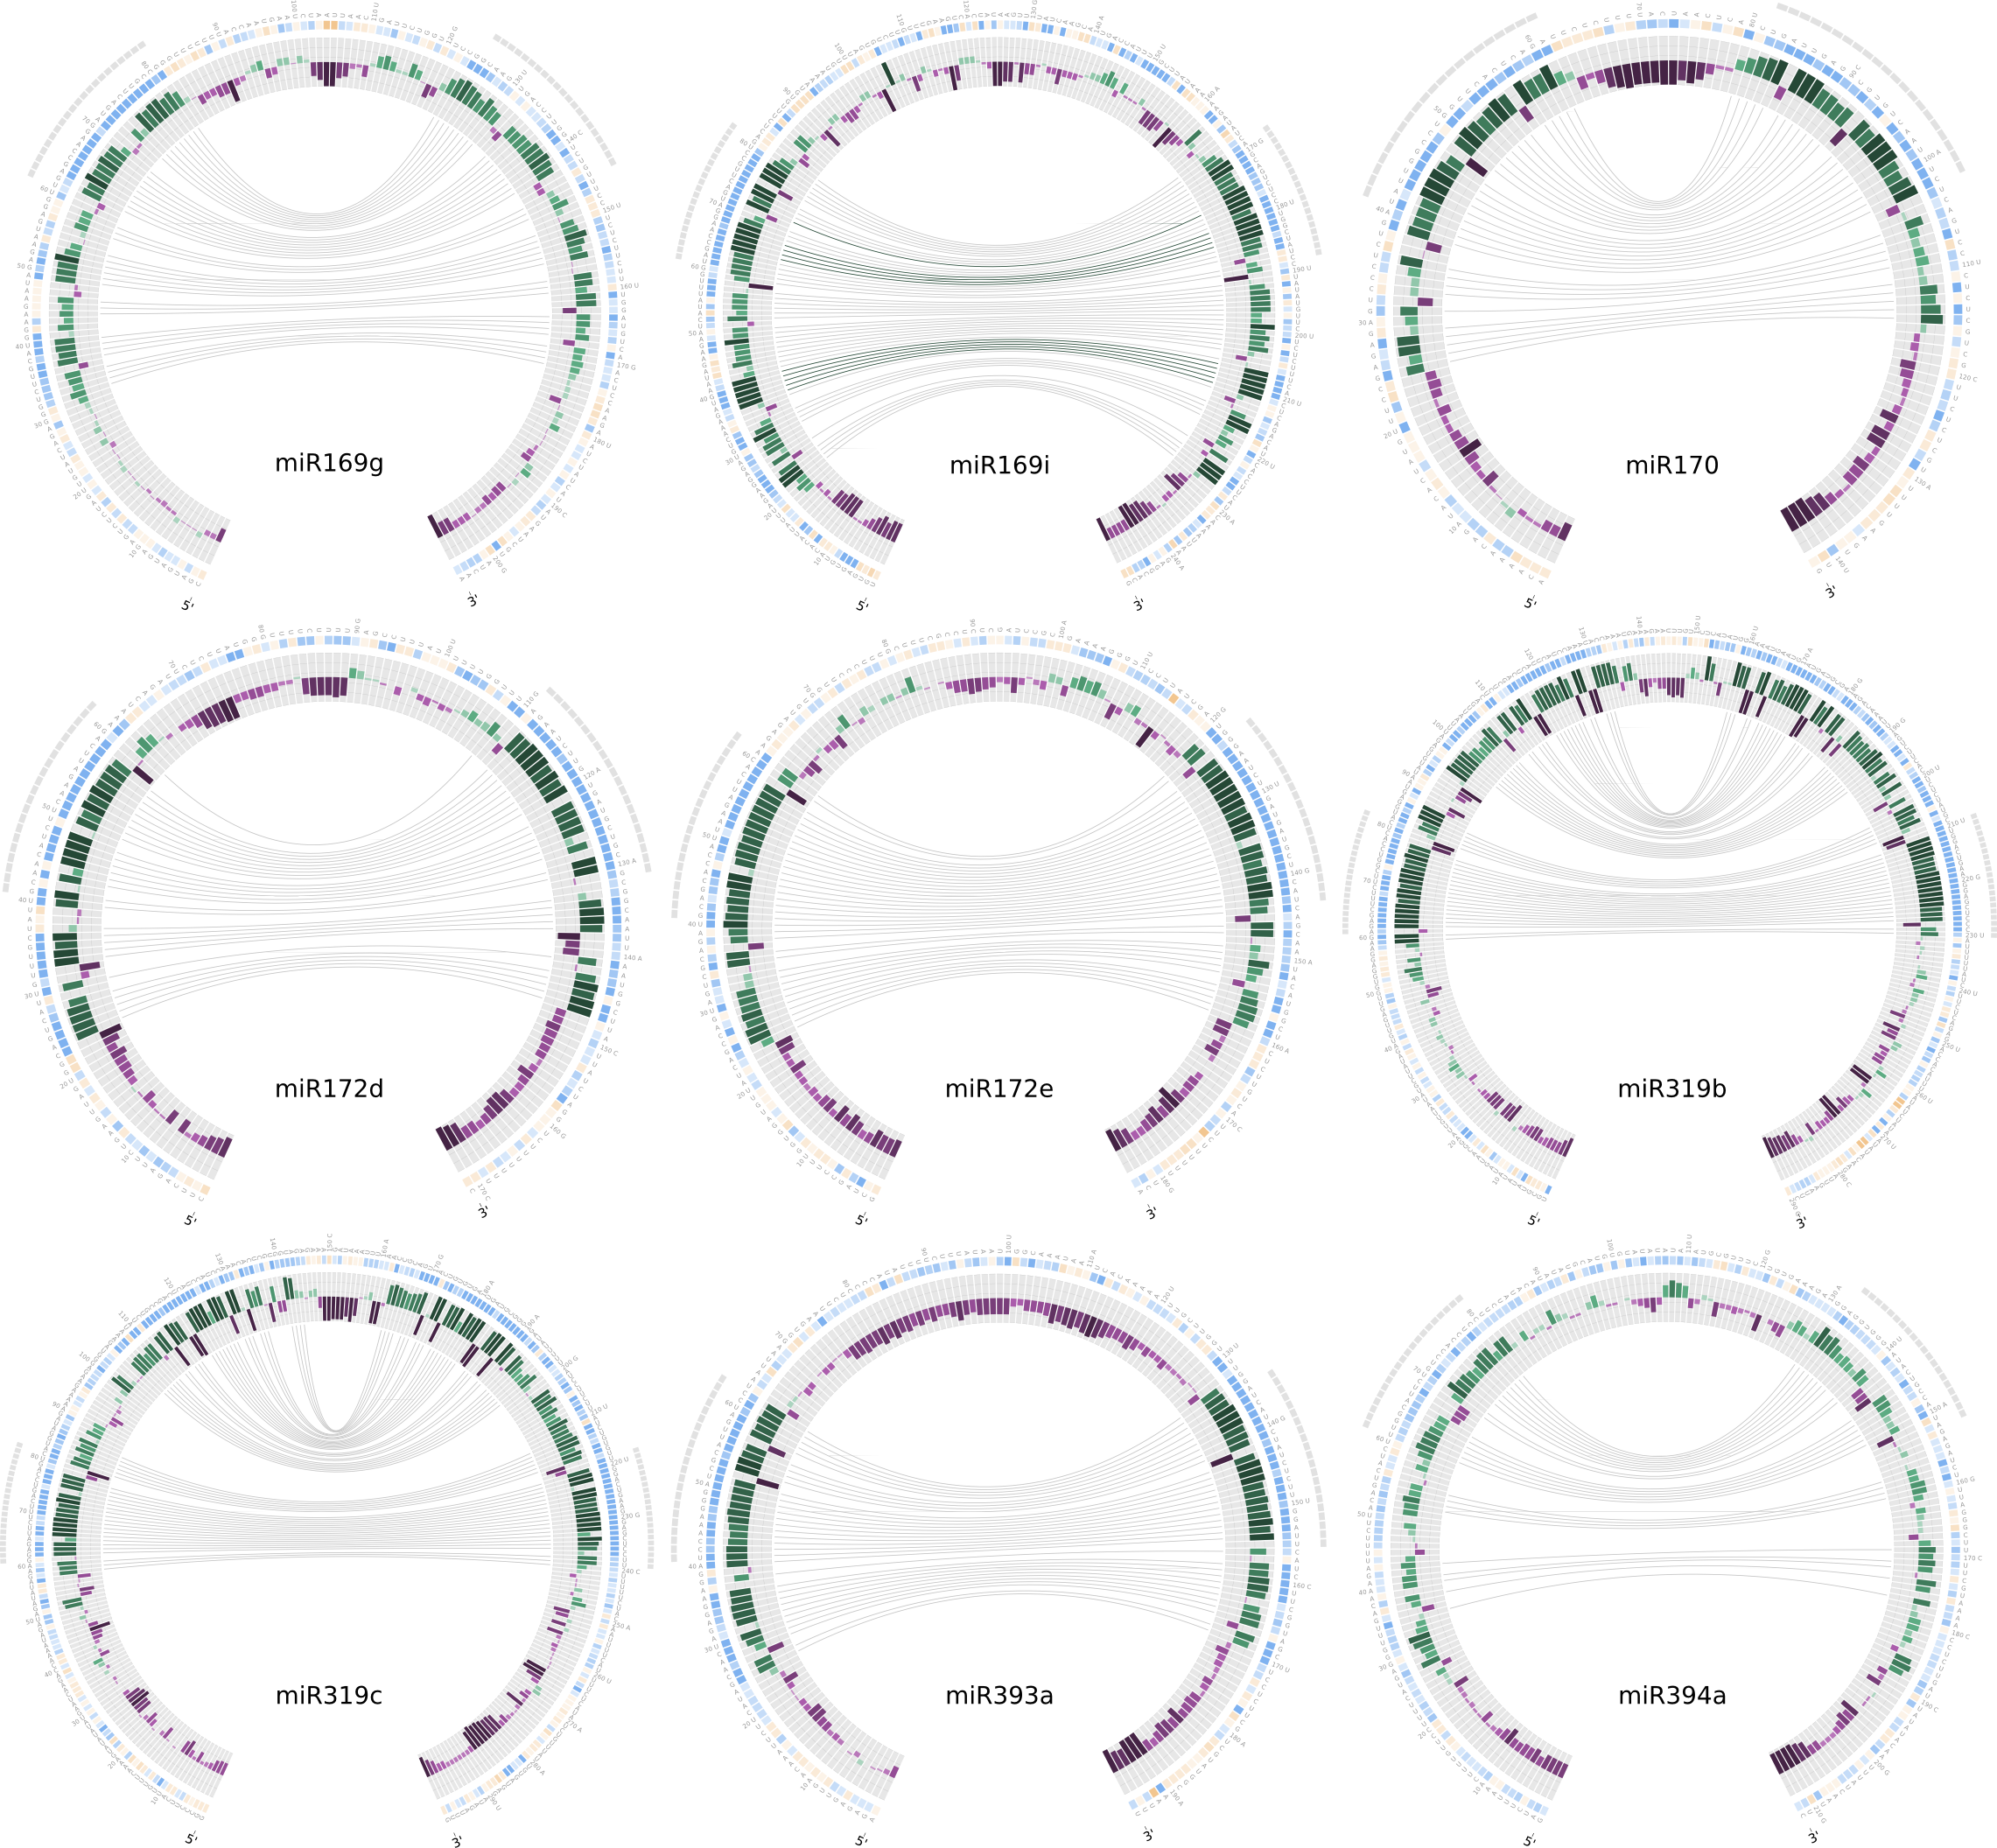
\includegraphics[width=1.3\textwidth]{circos_all_03.png}
        \caption[Circos de dicotiledóneas (en más de 20 especies). 3/5]{
        \textbf{Circos de dicotiledóneas donde se detectan ortólogos en más de 20 especies de las 30 analizadas.}
        Fig 3/5.
        }
        \label{fig:circos_all_03}
    \end{figure}
\end{landscape}

\begin{landscape}
    \begin{figure}[htbp!] 
        \centering    
        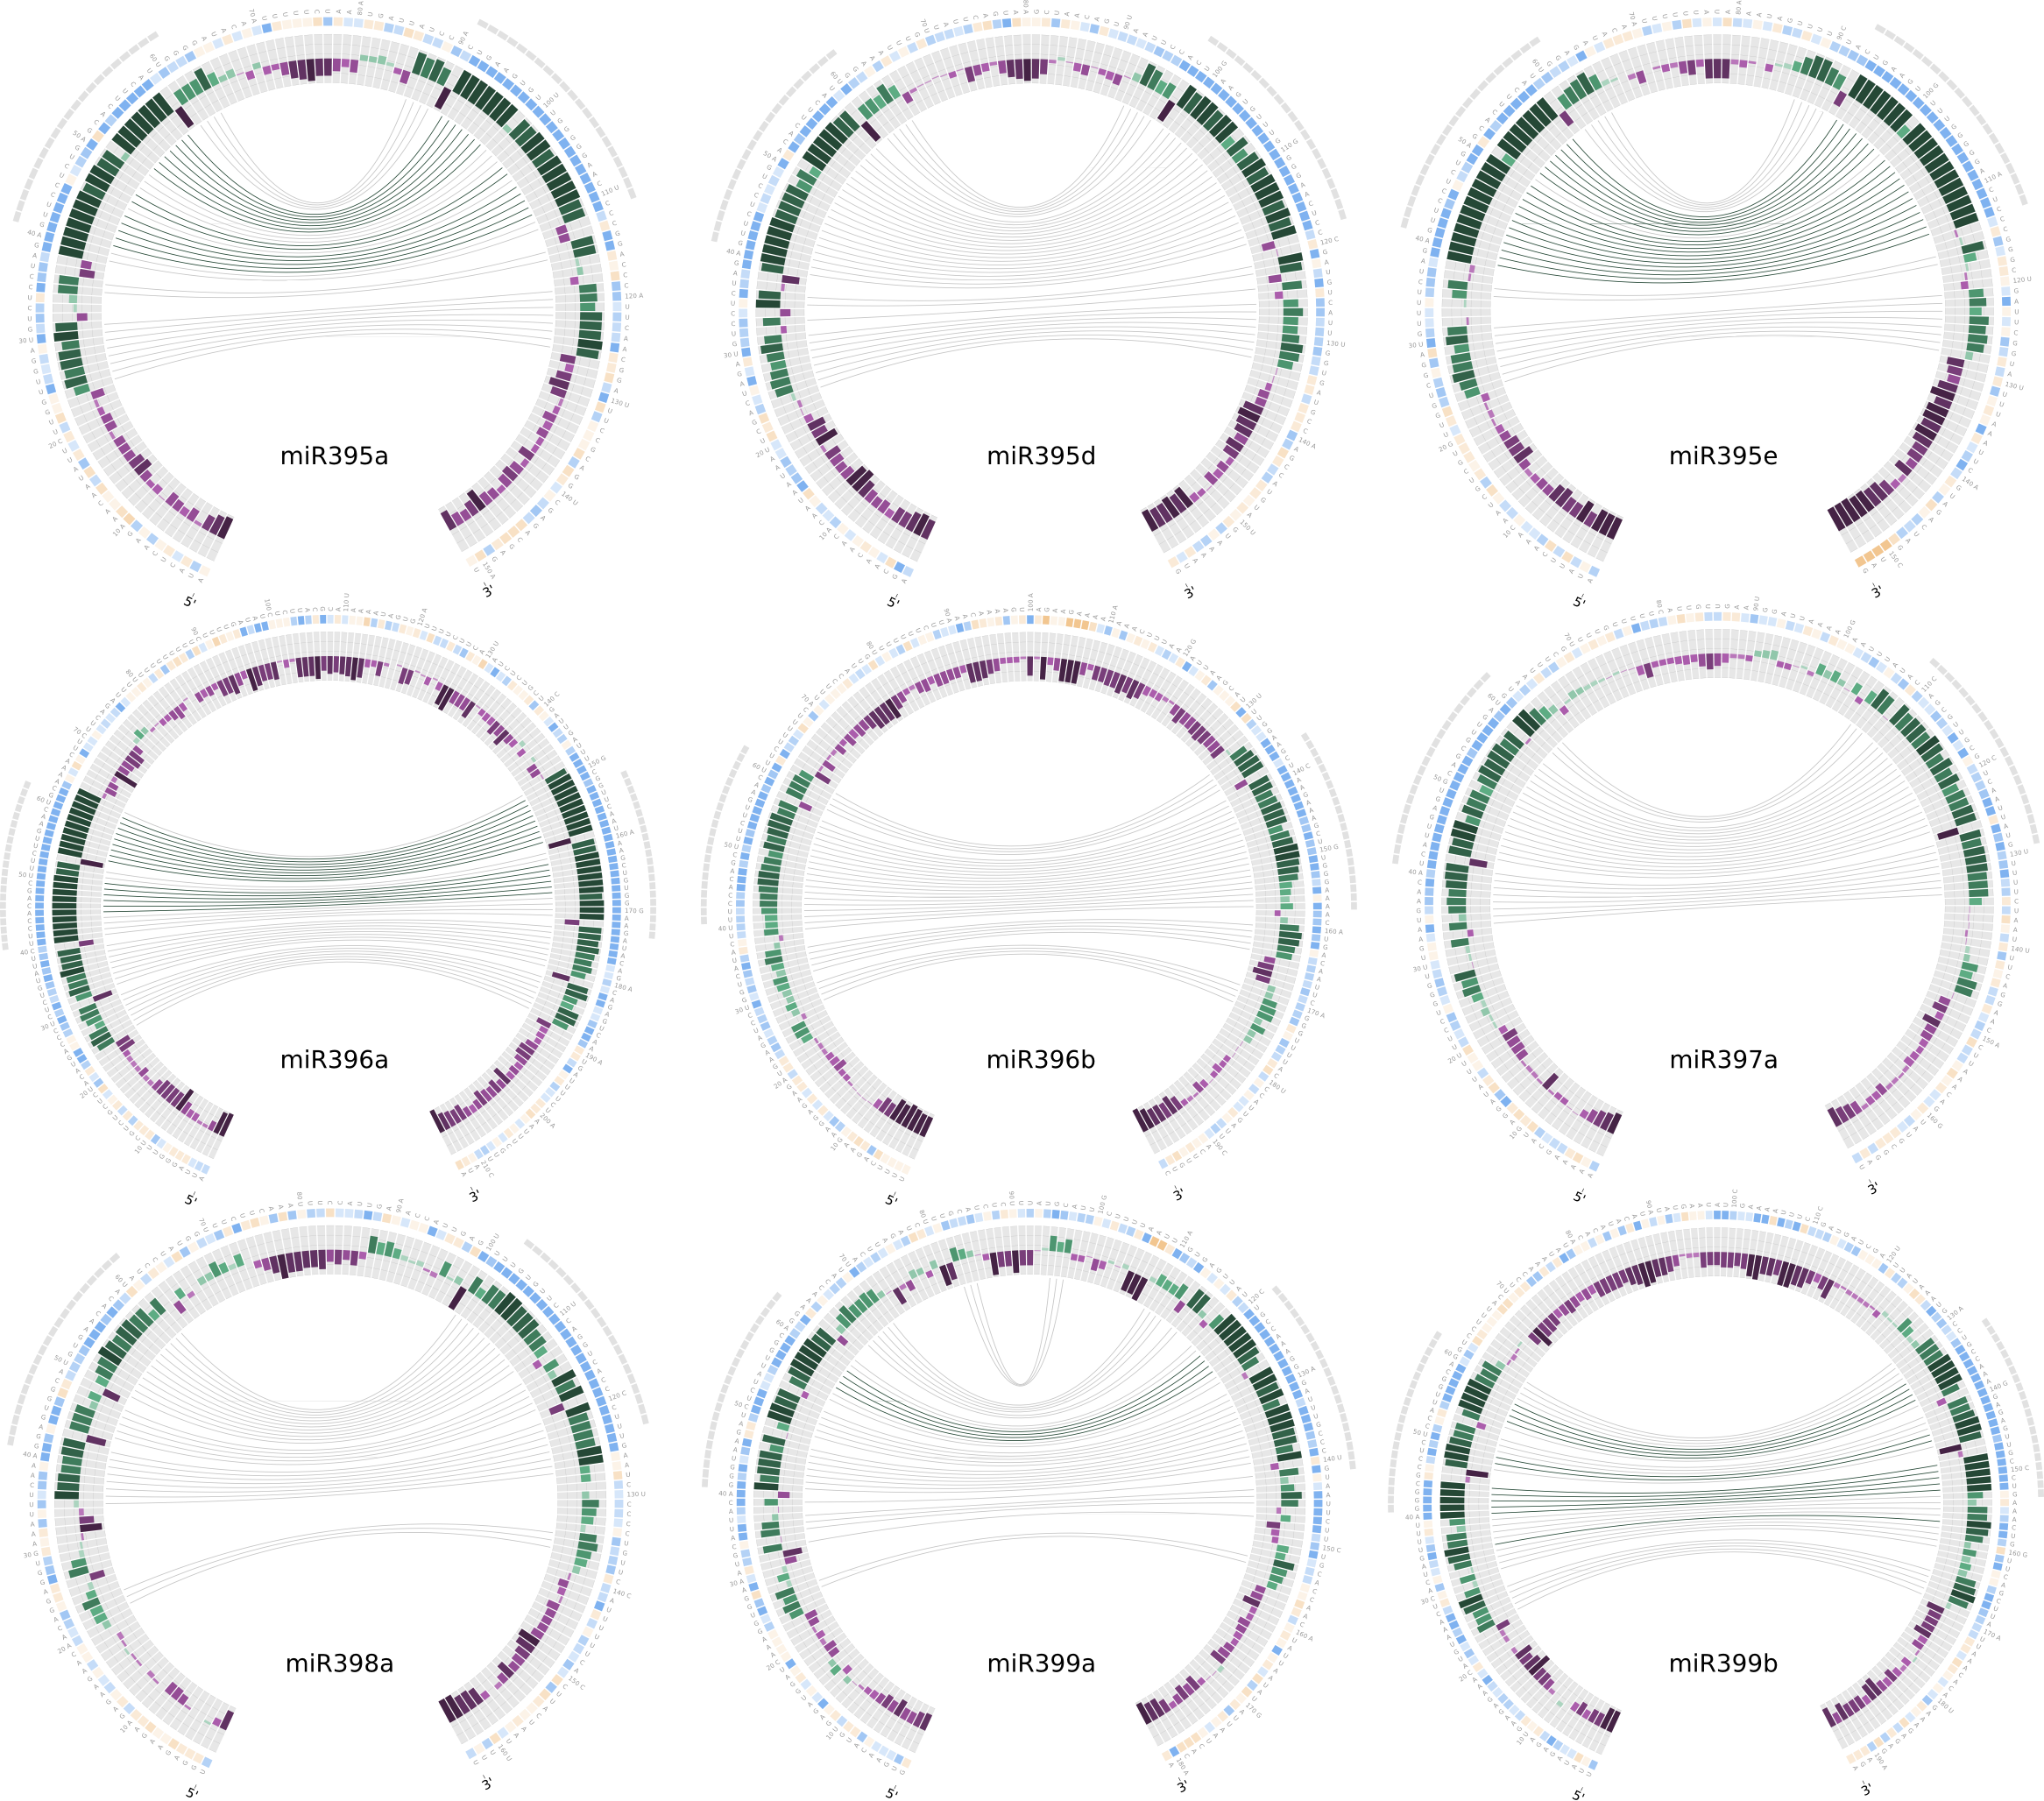
\includegraphics[width=1.3\textwidth]{circos_all_04.png}
        \caption[Circos de dicotiledóneas (en más de 20 especies). 4/5]{
        \textbf{Circos de dicotiledóneas donde se detectan ortólogos en más de 20 especies de las 30 analizadas.}
        Fig 4/5.
        }
        \label{fig:circos_all_04}
    \end{figure}
\end{landscape}

\begin{landscape}
    \begin{figure}[htbp!] 
        \centering    
        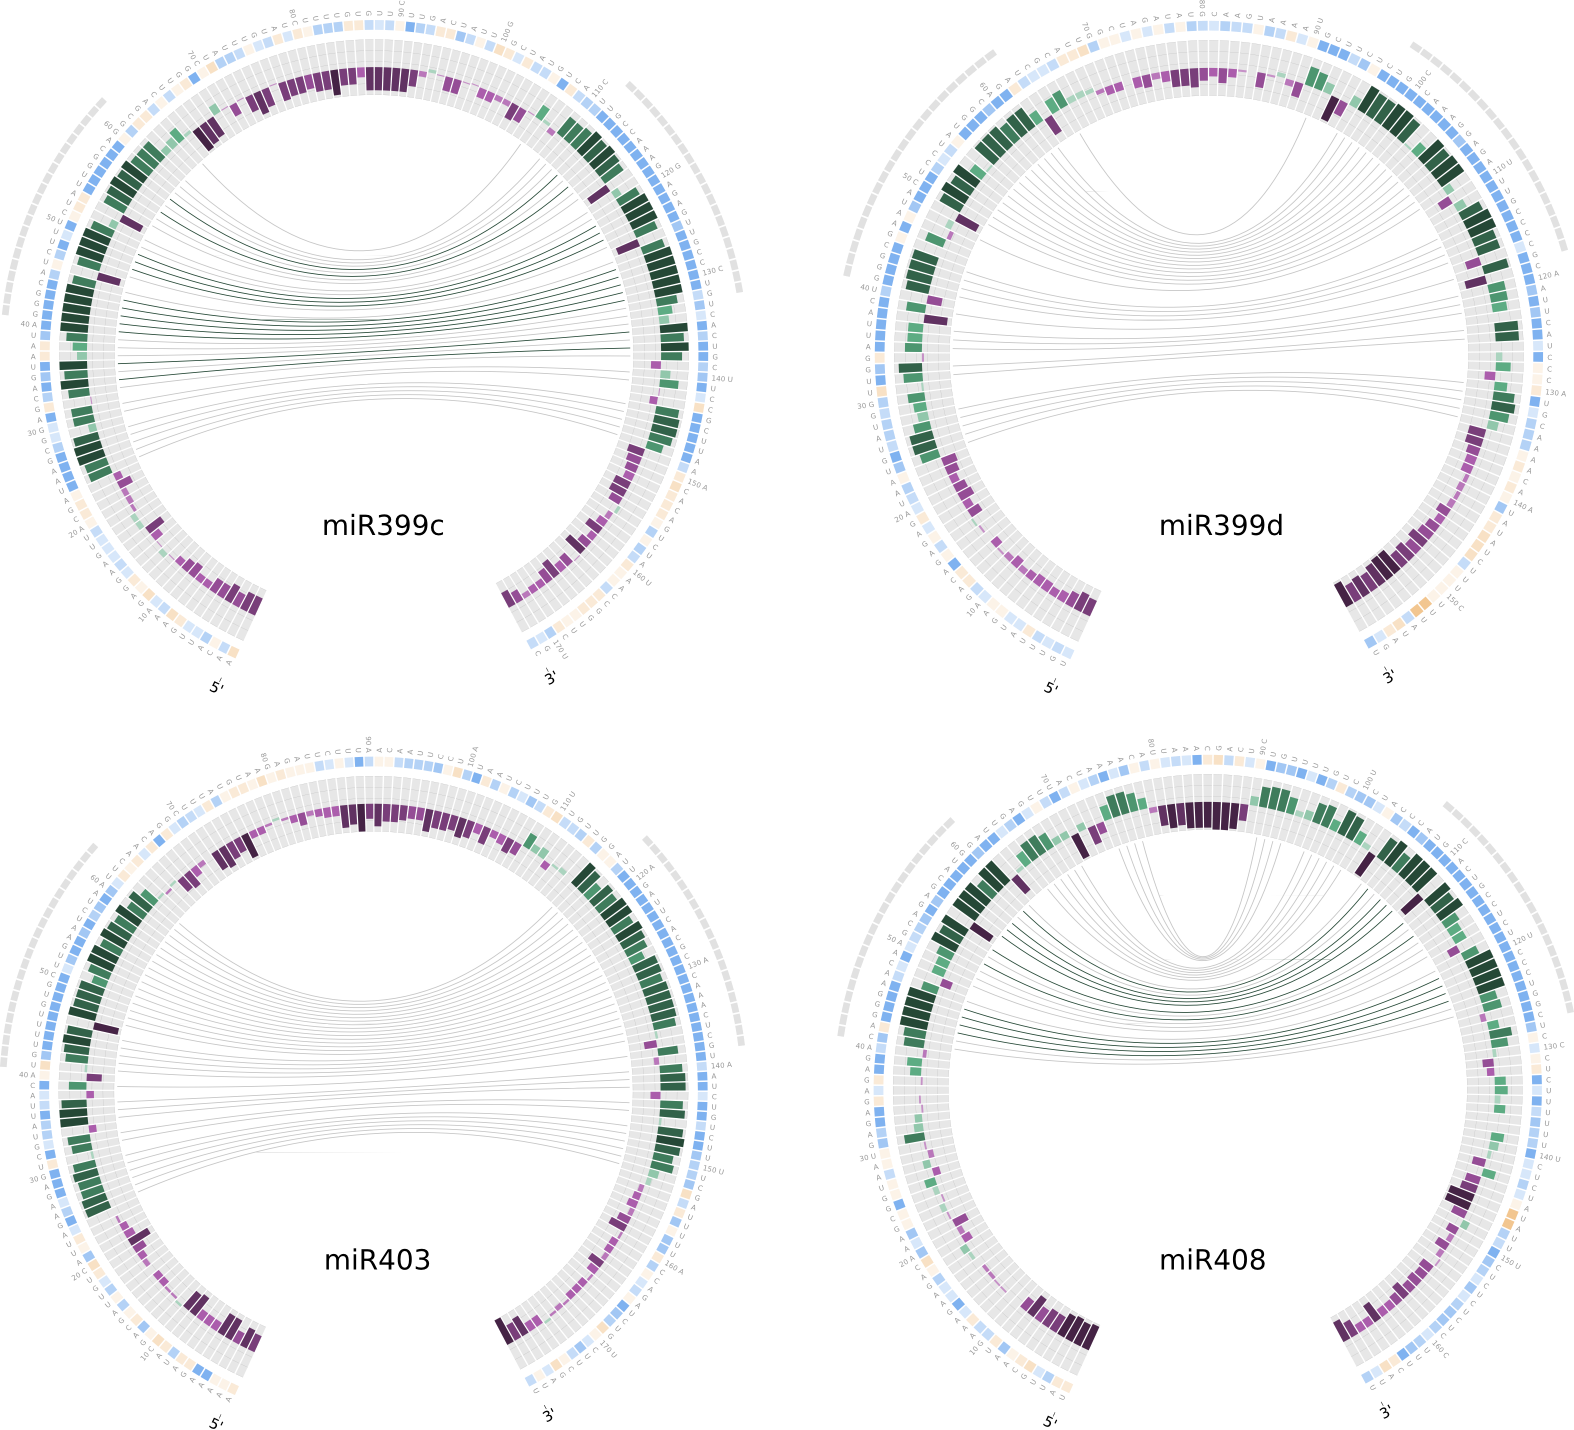
\includegraphics[width=1.3\textwidth]{circos_all_05.png}
        \caption[Circos de dicotiledóneas (en más de 20 especies). 5/5]{
        \textbf{Circos de dicotiledóneas donde se detectan ortólogos en más de 20 especies de las 30 analizadas.}
        Fig 5/5.
        }
        \label{fig:circos_all_05}
    \end{figure}
\end{landscape}


\begin{table}[htbp!]
\tiny
\centering
\caption{Genes blanco validados de familias miARNs conservados en plantas}
\label{table:NAR_table_S3}
\begin{tabular}{ccc}
\textbf{microRNA}      & \textbf{Target}       & \textbf{ID}        \\
miR156/miR157 & SPL          & At1g27370 \\
miR156/miR157 & SPL          & At1g53160 \\
miR156/miR157 & SPL          & At2g33810 \\
miR156/miR157 & SPL          & At3g15270 \\
miR156/miR157 & SPL          & At5g43270 \\
miR156/miR157 & SPL          & At1g69170 \\
miR156/miR157 & SPL          & At2g42200 \\
miR156/miR157 & SPL          & At3g57920 \\
miR156/miR157 & SPL          & At5g50670 \\
miR159/miR319 & TCP          & At1g30210 \\
miR159/miR319 & TCP          & At1g53230 \\
miR159/miR319 & TCP          & At2g31070 \\
miR159/miR319 & MYB          & At3g11440 \\
miR159/miR319 & TCP          & At3g15030 \\
miR159/miR319 & TCP          & At4g18390 \\
miR159/miR319 & MYB          & At5g06100 \\
miR159/miR319 & MYB          & At2g26950 \\
miR159/miR319 & MYB          & At2g32460 \\
miR159/miR319 & MYB          & At5g55020 \\
miR160        & ARF          & At1g77850 \\
miR160        & ARF          & At2g28350 \\
miR160        & ARF          & At4g30080 \\
miR162        & DCL          & At1g01040 \\
miR164        & NAC          & At1g56010 \\
miR164        & NAC          & At3g15170 \\
miR164        & NAC          & At5g07680 \\
miR164        & NAC          & At5g53950 \\
miR164        & NAC          & At5g61430 \\
miR164        & NAC          & At3g12977 \\
miR164        & NAC          & At5g39610 \\
miR166/miR165 & HD-ZIPIII    & At1g30490 \\
miR166/miR165 & HD-ZIPIII    & At1g52150 \\
miR166/miR165 & HD-ZIPIII    & At2g34710 \\
miR166/miR165 & HD-ZIPIII    & At5g60690 \\
miR166/miR165 & HD-ZIPIII    & At4g32880 \\
miR167        & ARF          & At1g30330 \\
miR167        & ARF          & At5g37020 \\
miR168        & AGO          & At1g48410 \\
miR169        & HAP2         & At1g17590 \\
miR169        & HAP2         & At1g54160 \\
miR169        & HAP2         & At1g72830 \\
miR169        & HAP2         & At3g05690 \\
miR169        & HAP2         & At3g20910 \\
miR169        & HAP2         & At5g06510 \\
miR170/miR171 & SCL          & At2g45160 \\
miR170/miR171 & SCL          & At3g60630 \\
miR170/miR171 & SCL          & At4g00150 \\
miR172        & AP2          & At2g28550 \\
miR172        & AP2          & At4g36920 \\
miR172        & AP2          & At5g60120 \\
miR172        & AP2          & At5g67180 \\
miR172        & AP2          & At2g39250 \\
miR172        & AP2          & At3g54990 \\
miR390/miR391 & TAS3         & At3g17185 \\
miR390/miR391 & TAS3         & At5g49615 \\
miR390/miR391 & TAS3         & At5g57735 \\
miR393        & TIR1/AFB     & At1g12820 \\
miR393        & bHLH         & At3g23690 \\
miR393        & TIR1/AFB     & At3g26810 \\
miR393        & TIR1/AFB     & At3g62980 \\
miR393        & TIR1/AFB     & At4g03190 \\
miR394        & F-Box        & At1g27340 \\
miR395        & APS          & At3g22890 \\
miR395        & AST          & At5g10180 \\
miR395        & APS          & At5g43780 \\
miR395        & APS          & At4g14680 \\
miR396        & GRF          & At2g22840 \\
miR396        & GRF          & At2g36400 \\
miR396        & GRF          & At2g45480 \\
miR396        & GRF          & At4g24150 \\
miR396        & GRF          & At4g37740 \\
miR396        & GRF          & At5g53660 \\
miR396        & GRF          & At3g52910 \\
miR397        & LAC          & At2g29130 \\
miR397        & LAC          & At2g38080 \\
miR397        & LAC          & At5g60020 \\
miR398        & CSD          & At1g08830 \\
miR398        & CSD          & At2g28190 \\
miR398        & CytC oxidase & At3g15640 \\
miR399        & E2-UBC       & At2g33770 \\
miR399        & E2-UBC       & At2g33770 \\
miR408        & LAC          & At2g30210 \\
mir408        & PLC          & At2g02850 \\
miR827        & SPX          & At1g02860
\end{tabular}
\end{table}

\begin{table}[htbp!]
\tiny
\centering
\caption{Mecanismos de procesamiento de miARNs conservados en \textit{A. thaliana}.}
\label{table:mecanismos}
\begin{tabular}{ll}
\textbf{miARN} & \textbf{Mecanismo}        \\
miR156a        & Corto de loop a base      \\
miR156b        & Corto de loop a base      \\
miR156c        & Corto de loop a base      \\
miR156d        & Corto de loop a base      \\
miR156e        & Corto de loop a base      \\
miR156h        & Corto de loop a base      \\
miR157a        & Corto de loop a base      \\
miR157b        & Corto de loop a base      \\
miR157c        & Corto de loop a base      \\
miR159a        & Secuencial de loop a base \\
miR159b        & Secuencial de loop a base \\
miR160a        & Corto de loop a base      \\
miR160b        & Corto de loop a base      \\
miR160c        & Corto de loop a base      \\
miR162a        & Corto de loop a base      \\
miR164b        & Corto de base a loop      \\
miR164c        & Corto de base a loop      \\
miR165a        & Corto de base a loop      \\
miR165b        & Corto de base a loop      \\
miR166a        & Corto de base a loop      \\
miR166b        & Corto de base a loop      \\
miR166f        & Corto de base a loop      \\
miR167a        & Corto de base a loop      \\
miR167b        & Corto de base a loop      \\
miR167c        & Corto de base a loop      \\
miR167d        & Corto de base a loop      \\
miR168a        & Corto de base a loop      \\
miR168b        & Corto de base a loop      \\
miR169a        & Corto de base a loop      \\
miR169b        & Secuencial de base a loop \\
miR169d        & Secuencial de base a loop \\
miR169e        & Secuencial de base a loop \\
miR169f        & Secuencial de base a loop \\
miR169h        & Secuencial de base a loop \\
miR169i        & Secuencial de base a loop \\
miR169j        & Secuencial de base a loop \\
miR169k        & Secuencial de base a loop \\
miR169l        & Secuencial de base a loop \\
miR169m        & Secuencial de base a loop \\
miR169n        & Secuencial de base a loop \\
miR170         & Corto de base a loop      \\
miR171a        & Corto de base a loop      \\
miR171b        & Corto de loop a base      \\
miR171c        & Corto de loop a base      \\
miR172a        & Corto de base a loop      \\
miR172b        & Corto de base a loop      \\
miR172c        & Corto de base a loop      \\
miR172d        & Corto de base a loop      \\
miR172e        & Corto de base a loop      \\
miR319a        & Secuencial de loop a base \\
miR319b        & Secuencial de loop a base \\
miR319c        & Secuencial de loop a base \\
miR390a        & Corto de base a loop      \\
miR390b        & Corto de base a loop      \\
miR391         & Corto de base a loop      \\
miR393a        & Corto de base a loop      \\
miR393b        & Corto de base a loop      \\
miR394a        & Secuencial de base a loop \\
miR394b        & Secuencial de base a loop \\
miR395a        & Corto de base a loop      \\
miR395b        & Corto de base a loop      \\
miR395c        & Corto de base a loop      \\
miR395d        & Corto de base a loop      \\
miR395f        & Corto de base a loop      \\
miR396a        & Corto de base a loop      \\
miR396b        & Corto de base a loop      \\
miR397a        & Corto de base a loop      \\
miR397b        & Corto de base a loop      \\
miR397c        & Corto de base a loop      \\
miR398b        & Corto de base a loop      \\
miR398c        & Corto de base a loop      \\
miR399a        & Corto de base a loop      \\
miR399b        & Corto de base a loop      \\
miR399c        & Corto de base a loop      \\
miR399d        & Corto de base a loop      \\
miR408         & Corto de base a loop      \\
miR827         & Corto de base a loop     
\end{tabular}
\end{table}
